\chapter{Methodology\label{cha:methodology}}
In this chapter, we describe how we design and implement the experiments with
\acrshort{gan}s to achieve the objective of the Thesis.

\section{Our \acrshort{gan}s }
The main contribution of the Thesis is to use the concept of \acrshort{gan} to
adversarially train a generative model which can produce a reasonable depth-map of a
given 2D image of a particular object. The model is expected to be able to
understand the 3D properties of images of single objects. Because of its tasks, we call
this one the "Depth-GAN".

In addition, we also train another \acrshort{gan} to learn the 3D knowledge in another
dimension, the pose estimator. This \acrshort{gan}'s job is to generate a 2D image of the
same given object in another pose. It is expected to be able to rotate, in 3D space, the
object by a particular angle while being conditioned on the object 2D image and its
corresponding depth-map. We call this one the "Pose-GAN"

\subsection{Network Architecture}
We inherit the architecture from \acrshort{pix} with only some occasional modifications in
the input and output layers because our experiments, especially the first one which
generates depth-maps from an RGB image, is very close to their settings. 

The Generator is basically an U-Net \cite{u_net}, an encoder-decoder with skip
connections between every decoder layer and the corresponding encoder layer. The intuition
behind this is that, there are relevant information between the input and the output.
Especially the mirrors in the encoder part and the decoder part share the same resolution
and same level of encoding. Therefore, letting them connect directly is a good idea.
Figure~\ref{fig:u_net} visualizes the architectures of both a standard Encoder-Decoder and
U-Net.

Similarly, the Discriminator is also a Convolution-Batch-Norm-ReLu structure. It
implements an idea which the authors call "PatchGAN", where an image are divided to some
$N \times N$ patches and the network only judges the real-fake properties of each patch.
The final decision is averaged over the single-patch decisions. The rest of its job are
exactly the same as a normal binary classifier.

\begin{figure}[h]
	\centering
	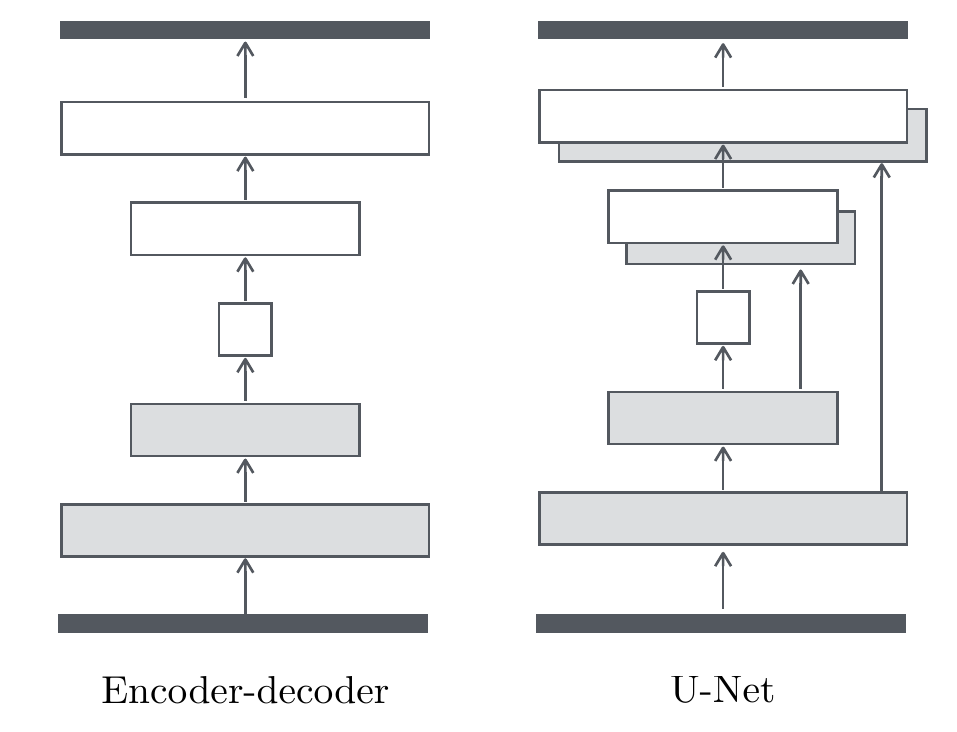
\includegraphics[width=0.8\linewidth]{u_net}
	\caption{Standard Encoder-Decoder and U-Net architectures}
	\label{fig:u_net}
\end{figure}


\subsection{Data}
As being mentioned above, in this Thesis we focus on 2 tasks on \acrshort{gan}: learning
to generate depth information and learning to generate another pose of an object. As we
are doing image-to-image translation tasks, we call the conditional image the "input", the
to-be-generated image the "output", and the ground-truth the "target". The Generator is
supposed to make the output as close to the target as possible, while the Discriminator
still tries its best to tell them apart.

In the first \acrshort{gan}, we line the Washington RGBD dataset up by putting every RGB
image along with the corresponding depth-map. Here the RGB is the input, the generated
depth-map is the output, and the . As the RGB image is an 8-bit one and the depth-map is
16-bit, we have to manipulate the data loading process to make sure that we have the
correct forms. A wrong manipulation can lead to a great loss of information.

In the additional \acrshort{gan} where we want to learn to generate a different pose of
the same object, we use both the RGB frame and the corresponding (real) depth-map as the
input condition to \acrshort{gan}, to both the Generator and Discriminator. The depth-map
is pre-processed and attached to the RGB frame as the 4th dimension, along with the three
color channels. This \acrshort{gan} will then use this information to produce a normal
3-channel RGB image of the same object, but in another pose. The Discriminator's task is
to classify this rotated image with the real image in that pose. Here the input is a
4-dimensional image, the output is an RGB, and the target is a real RGB image of that
pose.

For every frame, we choose the target pose of the 10th frame in the video sequence, which
is equivalent to a rotation of roughly 20\degree. We do that for several reasons. First,
there are subtle differences and errors among different camera scans, which makes choosing
an exact pose, such as 15\degree or 20\degree, unrealistic. Second, as we also have a
complex stratified Train-Test split which will be explained in details in section
\ref{sec:train_test_split}, we would like to make sure that the target pose of every input
frame should be in the same part of the split. A combination of an input from the training
split and a target from the test split can lead to dangerous bias in evaluation, for both
the \acrshort{gan} and the baseline classifier. Because we pick every 5th frame from every
instance to be in the test set, choosing the 10th frame as the target makes sure that the
rotated pose is in the same train-test split. Third and finally, a target rotation of
roughly 20\degree is a reasonable choice as it is big enough to observe a clear rotation
but still contains many similar details as the input, which makes the task more feasible.

For all types of \acrshort{gan}s that we are working with, the Generator produces the
Output, and the Discriminator reads both the Output and the Target and try its best to
classify the two, while both of them are conditioned on the Input. To simplify the
language, from this point we will sometimes refer both of them (i.e. the Generator and the
Discriminator) to \acrshort{gan} only. For instance, the statement "The \acrshort{gan} reads
image A and generates image B" is equivalent to "The Generator generates image B and the
Discriminator tries to distinguish image B and a target B', while both of them are
conditioned on image A"

\subsection{Manipulation of depth missing values }
Due to technical limitations, there are corners that the sensors cannot capture the depth
information. Those values are represented as 0's in the depth-maps. If we just keep the
depth-maps as they are and feed them to the Discriminator, the \acrshort{gan} will learn
the missing value patterns and will probably somehow generate a representation of missing
values according to its understanding. This is not really what we expect; thus,
interpolating the missing values can be a good pre-processing step.

In this Thesis, we use the colorization method from a toolbox from NYU \cite{nyu_dataset},
which applies the colorization method from Levin et al. \cite{levin_colorization}. The algorithm
uses the RGB information to infer the depth values of the missing points. The
details of the optimization method can be found in the paper \cite{levin_colorization}.

\section{Baseline task}
For the baseline task, we keep most of the architecture of the 2-channel network proposed
by Eitel et al. Our implementation makes some changes on the Manipulation of the depth
missing values and the way we train the network.

In the paper, the authors propose a noise injection method to the depth-maps in the
training process. The idea is too mimic the missing values patterns (the 0 values in the
maps) so that the classifier becomes robust towards them. In other words, missing values
are considered as noise in data. In our implementation, because we also remove those
missing values from the \acrshort{gan} training process for some reasons that we have
explained in the previous section, we also do the same to the classification. Basically,
we would like the data we use to train our \acrshort{gan} and the classifier to have
identical formats. It turns out that our approach gives slightly better classification
accuracies, which we will discuss in details in chapter \ref{chap:evaluation}.

As our approach of handling the missing values already gives better accuracies on the
original data, we do not perform fine-tuning the AlexNet channels as the authors did. A
benefit of not fine-tuning is that we can utilize the AlexNet representations for
different training rounds without re-doing back-propagation throughout the entire 9 layers
of the 2-channel network. In fact, we only train the 2 last layers for most of the
experiments.

\section{Evaluation Method}
\subsection{Train-Test split methodology\label{sec:train_test_split}}
As we are working on 2 Deep Learning tasks and the dataset contains many details in
different layers, a naive random Train-Test split is not the optimal approach. For this
purpose, we design a more stratified split, which is demonstrated in
Figure~\ref{fig:gan_train_test_split}.

For the baseline classifier, we split the data using the same strategy as in Eitel et al
\cite{eitel}, the work we refer to. In each instance, every fifth frame is sampled
and in every object, one instance is randomly and completely taken out. This gives us
about 138000 items for training and about 69000 items for testing.  We also perform the
10-cross-validation splits introduced in Lai et al \cite{washington_rgbd}. That is, each of the
lifting angle sequence is divided in to 3 sub-sequences (let us recall that each instance
in the Washington RGBD dataset is recorded in 3 different lifting angles: 30, 45 and 60
degrees).  Among those 9 sub-sequences, two are randomly added to the evaluation set. In
total, each experiment is done by using about 128000 items for training and about 78000
items for testing.

For \acrshort{gan} training, as we aim to use the \acrshort{gan} results to substitute
the real data in training the baseline classifier, we also have to design an additional
train-test split. The evaluation set generated from the previous strategy is left alone
without any further modification. Instead, we randomly split the classifier's training set
in different scales: 50-50, 25-75 and 10-90. The left portions are used for training the
\acrshort{gan} and the right portions are used to evaluate it, of which the results will
substitute the corresponding real items in the training set of the classifier. In this
way, we make sure that:

\begin{itemize}
	\item \acrshort{gan} has not seen the items it is generating samples from. In
		other words, \acrshort{gan} is in evaluation mode when being used for training the
		baseline classifier. This is important because we cannot directly use the training output
		from \acrshort{gan} to train the baseline classifier, which is bias and encourages over-fitting.
	\item We can objectively compare the classification results trained from similar
		amount of data but with different portions of real-fake components. In this way,
		we can see how \acrshort{gan} contributes to the classification accuracies in
		different scales.
\end{itemize}

\begin{figure}[h]
	\centering
	\includegraphics[width=\linewidth]{img/gan_train_test_split}
	\caption{Our stratified Train-Test split for evaluating the depth-maps generation with
		\acrshort{gan}. The Stratified-Sampled Training set is split into a GAN Training
		Set and GAN Test Set with different proportions.}
	\label{fig:gan_train_test_split}
\end{figure}

However, this is worth to know that this approach also has a drawback. The comparisons of
different \acrshort{gan} training setups are not entirely fair because the amounts of data
used in training the \acrshort{gan} are different. For instance, if we would like to have
90\% of \acrshort{gan} data to train the classifier, we can use only the remaining 10\% of
the data to train the \acrshort{gan} to make sure that the generated data has not been
seen by \acrshort{gan} before. However, if we keep only 50\% of \acrshort{gan} data in the
classifier's training set, we can use up to 50\% of the remaining data to train it, which
potentially results in a stronger \acrshort{gan}. 
